% !TeX spellcheck = hu_HU
% !TeX encoding = UTF-8
% !TeX program = xelatex
% TODO Change language to en_GB (recommended) or en_US for English documents
\documentclass[11pt,a4paper,oneside]{report}             % Single-side
%\documentclass[11pt,a4paper,twoside,openright]{report}  % Duplex

% thanks to http://tex.stackexchange.com/a/47579/71109
\usepackage{ifxetex}
\usepackage{ifluatex}
\newif\ifxetexorluatex % a new conditional starts as false
\ifnum 0\ifxetex 1\fi\ifluatex 1\fi>0
   \xetexorluatextrue
\fi

\ifxetexorluatex
  \usepackage{fontspec}
\else
  \usepackage[T1]{fontenc}
  \usepackage[utf8]{inputenc}
  \usepackage[lighttt]{lmodern}
\fi

\usepackage[english,magyar]{babel} % Alapértelmezés szerint utoljára definiált nyelv lesz aktív, de később külön beállítjuk az aktív nyelvet.

%\usepackage{cmap}
\usepackage{amsfonts,amsmath,amssymb} % Mathematical symbols.
%\usepackage[ruled,boxed,resetcount,linesnumbered]{algorithm2e} % For pseudocodes. % beware: this is not compatible with LuaLaTeX, see http://tex.stackexchange.com/questions/34814/lualatex-and-algorithm2e
\usepackage{booktabs} % For publication quality tables for LaTeX
\usepackage{graphicx}

%\usepackage{fancyhdr}
%\usepackage{lastpage}

\usepackage{anysize}
%\usepackage{sectsty}
\usepackage{setspace} % For setting line spacing

\usepackage[unicode]{hyperref} % For hyperlinks in the generated document.
\usepackage{xcolor}
\usepackage{listings} % For source code snippets.

\usepackage[amsmath,thmmarks]{ntheorem} % Theorem-like environments.

\usepackage[hang]{caption}

\singlespacing

\newcommand{\selecthungarian}{
	\selectlanguage{magyar}
	\setlength{\parindent}{2em}
	\setlength{\parskip}{0em}
	\frenchspacing
}

\newcommand{\selectenglish}{
	\selectlanguage{english}
	\setlength{\parindent}{0em}
	\setlength{\parskip}{0.5em}
	\nonfrenchspacing
	\renewcommand{\figureautorefname}{Figure}
	\renewcommand{\tableautorefname}{Table}
	\renewcommand{\partautorefname}{Part}
	\renewcommand{\chapterautorefname}{Chapter}
	\renewcommand{\sectionautorefname}{Section}
	\renewcommand{\subsectionautorefname}{Section}
	\renewcommand{\subsubsectionautorefname}{Section}
}

\usepackage[numbers]{natbib}
\usepackage{xspace}

% saját vackok amik kellhetnek
% todo package
\usepackage{todonotes}
\usepackage{dirtree}


%TODO Set the main variables
\newcommand{\vikszerzoVezeteknev}{Koloszár}
\newcommand{\vikszerzoKeresztnev}{Gergely}

\newcommand{\vikkonzulensAMegszolitas}{~}
\newcommand{\vikkonzulensAVezeteknev}{Bányász}
\newcommand{\vikkonzulensAKeresztnev}{Gábor}

\newcommand{\vikkonzulensBMegszolitas}{}
\newcommand{\vikkonzulensBVezeteknev}{}
\newcommand{\vikkonzulensBKeresztnev}{}

\newcommand{\vikkonzulensCMegszolitas}{}
\newcommand{\vikkonzulensCVezeteknev}{}
\newcommand{\vikkonzulensCKeresztnev}{}

\newcommand{\vikcim}{Labirintus megoldó robot} % Cím
\newcommand{\viktanszek}{\bmeaut} % Tanszék
\newcommand{\vikdoktipus}{\msc} % Dokumentum típusa (\bsc vagy \msc)
\newcommand{\vikmunkatipusat}{diplomatervet} % a "hallgató nyilatkozat" részhez: szakdolgozatot vagy diplomatervet

%--------------------------------------------------------------------------------------
% TDK-specifikus változók
%--------------------------------------------------------------------------------------
\newcommand{\tdkszerzoB}{Második Szerző} % Második szerző neve; hagyd üresen, ha egyedül írtad a TDK-t.
\newcommand{\tdkev}{2014} % A dolgozat írásának éve (pl. "2014") (Ez OTDK-nál eltérhet az aktuális évtől.)

% További adatok az OTDK címlaphoz (BME-s TDK-hoz nem kell kitölteni)
\newcommand{\tdkevfolyamA}{IV} % Első szerző évfolyama, római számmal (pl. IV).
\newcommand{\tdkevfolyamB}{III} % Második szerző évfolyama, római számmal (pl. III).
\newcommand{\tdkkonzulensbeosztasA}{egyetemi tanár} % Első konzulens beosztása (pl. egyetemi docens)
\newcommand{\tdkkonzulensbeosztasB}{doktorandusz} % Második konzulens beosztása (pl. egyetemi docens)

\newcommand{\szerzoMeta}{\vikszerzoVezeteknev{} \vikszerzoKeresztnev} % egy szerző esetén
%\newcommand{\szerzoMeta}{\vikszerzoVezeteknev{} \vikszerzoKeresztnev, \tdkszerzoB} % két szerző esetén

%TODO Language configuration -- choose one
% Beállítások magyar nyelvű dolgozathoz
%--------------------------------------------------------------------------------------
% Elnevezések
%--------------------------------------------------------------------------------------
\newcommand{\bme}{Budapesti Műszaki és Gazdaságtudományi Egyetem}
\newcommand{\vik}{Villamosmérnöki és Informatikai Kar}

\newcommand{\bmemit}{Méréstechnika és Információs Rendszerek Tanszék}
\newcommand{\bmeaut}{Automatizálási és Alkalmazott Informatikai Tanszék}

\newcommand{\keszitette}{Készítette}
\newcommand{\konzulens}{Konzulens}

\newcommand{\bsc}{Szakdolgozat}
\newcommand{\msc}{Diplomaterv}
\newcommand{\tdk}{TDK dolgozat}
\newcommand{\bsconlab}{BSc Önálló laboratórium}
\newcommand{\msconlabi}{MSc Önálló laboratórium 1.}
\newcommand{\msconlabii}{MSc Önálló laboratórium 2.}

\newcommand{\pelda}{Példa}
\newcommand{\definicio}{Definíció}
\newcommand{\tetel}{Tétel}

\newcommand{\bevezetes}{Bevezetés}
\newcommand{\koszonetnyilvanitas}{Köszönetnyilvánítás}
\newcommand{\fuggelek}{Függelék}

% Opcionálisan átnevezhető címek
%\addto\captionsmagyar{%
%\renewcommand{\listfigurename}{Saját ábrajegyzék cím}
%\renewcommand{\listtablename}{Saját táblázatjegyzék cím}
%\renewcommand{\bibname}{Saját irodalomjegyzék név}
%}

\newcommand{\szerzo}{\vikszerzoVezeteknev{} \vikszerzoKeresztnev}
\newcommand{\vikkonzulensA}{\vikkonzulensAMegszolitas\vikkonzulensAVezeteknev{} \vikkonzulensAKeresztnev}
\newcommand{\vikkonzulensB}{\vikkonzulensBMegszolitas\vikkonzulensBVezeteknev{} \vikkonzulensBKeresztnev}
\newcommand{\vikkonzulensC}{\vikkonzulensCMegszolitas\vikkonzulensCVezeteknev{} \vikkonzulensCKeresztnev}

\newcommand{\selectthesislanguage}{\selecthungarian}

\bibliographystyle{huplain}

\def\lstlistingname{lista}

\newcommand{\appendixnumber}{6}  % a fofejezet-szamlalo az angol ABC 6. betuje (F) lesz

% Settings for English documents
%% %--------------------------------------------------------------------------------------
% Elnevezések
%--------------------------------------------------------------------------------------
\newcommand{\bme}{Budapest University of Technology and Economics}
\newcommand{\vik}{Faculty of Electrical Engineering and Informatics}

\newcommand{\bmemit}{Department of Measurement and Information Systems}
\newcommand{\bmeaut}{Department of Automation and Applied Informatics}

\newcommand{\keszitette}{Author}
\newcommand{\konzulens}{Advisor}

\newcommand{\bsc}{Bachelor's Thesis}
\newcommand{\msc}{Master's Thesis}
\newcommand{\tdk}{Scientific Students' Association Report}
\newcommand{\bsconlab}{BSc Project Laboratory}
\newcommand{\msconlabi}{MSc Project Laboratory 1}
\newcommand{\msconlabii}{MSc Project Laboratory 2}

\newcommand{\pelda}{Example}
\newcommand{\definicio}{Definition}
\newcommand{\tetel}{Theorem}

\newcommand{\bevezetes}{Introduction}
\newcommand{\koszonetnyilvanitas}{Acknowledgements}
\newcommand{\fuggelek}{Appendix}

% Optional custom titles
%\addto\captionsenglish{%
%\renewcommand*{\listfigurename}{Your list of figures title}
%\renewcommand*{\listtablename}{Your list of tables title}
%\renewcommand*{\bibname}{Your bibliography title}
%}

\newcommand{\szerzo}{\vikszerzoKeresztnev{} \vikszerzoVezeteknev}
\newcommand{\vikkonzulensA}{\vikkonzulensAMegszolitas\vikkonzulensAKeresztnev{} \vikkonzulensAVezeteknev}
\newcommand{\vikkonzulensB}{\vikkonzulensBMegszolitas\vikkonzulensBKeresztnev{} \vikkonzulensBVezeteknev}
\newcommand{\vikkonzulensC}{\vikkonzulensCMegszolitas\vikkonzulensCKeresztnev{} \vikkonzulensCVezeteknev}

\newcommand{\selectthesislanguage}{\selectenglish}

\bibliographystyle{plainnat}

\newcommand{\ie}{i.e.\@\xspace}
\newcommand{\Ie}{I.e.\@\xspace}
\newcommand{\eg}{e.g.\@\xspace}
\newcommand{\Eg}{E.g.\@\xspace}
\newcommand{\etal}{et al.\@\xspace}
\newcommand{\etc}{etc.\@\xspace}
\newcommand{\vs}{vs.\@\xspace}
\newcommand{\viz}{viz.\@\xspace} % videlicet
\newcommand{\cf}{cf.\@\xspace} % confer
\newcommand{\Cf}{Cf.\@\xspace}
\newcommand{\wrt}{w.r.t.\@\xspace} % with respect to
\newcommand{\approximately}{approx.\@\xspace}

\newcommand{\appendixnumber}{1}  % a fofejezet-szamlalo az angol ABC 1. betuje (A) lesz


%--------------------------------------------------------------------------------------
% Page layout setup
%--------------------------------------------------------------------------------------
% we need to redefine the pagestyle plain
% another possibility is to use the body of this command without \fancypagestyle
% and use \pagestyle{fancy} but in that case the special pages
% (like the ToC, the References, and the Chapter pages)remain in plane style

\pagestyle{plain}
\marginsize{35mm}{25mm}{25mm}{25mm} % tükörmargó,mindenhol 2.5 bal oldalt +1 cm kötés
\linespread{1.3}                    % másfeles sorköz

\setcounter{tocdepth}{3}
%\sectionfont{\large\upshape\bfseries}
\setcounter{secnumdepth}{3}

\sloppy % Margón túllógó sorok tiltása.
\widowpenalty=10000 \clubpenalty=10000 %A fattyú- és árvasorok elkerülése
\def\hyph{-\penalty0\hskip0pt\relax} % Kötőjeles szavak elválasztásának engedélyezése


%--------------------------------------------------------------------------------------
% Setup hyperref package
%--------------------------------------------------------------------------------------
\hypersetup{
    % bookmarks=true,          % show bookmarks bar?
    unicode=true,              % non-Latin characters in Acrobat's bookmarks
    pdftitle={\vikcim},        % title
    pdfauthor={\szerzoMeta},   % author
    pdfsubject={\vikdoktipus}, % subject of the document
    pdfcreator={\szerzoMeta},  % creator of the document
    pdfproducer={},            % producer of the document
    pdfkeywords={},            % list of keywords (separate then by comma)
    pdfnewwindow=true,         % links in new window
    colorlinks=true,           % false: boxed links; true: colored links
    linkcolor=black,           % color of internal links
    citecolor=black,           % color of links to bibliography
    filecolor=black,           % color of file links
    urlcolor=black             % color of external links
}


%--------------------------------------------------------------------------------------
% Set up listings
%--------------------------------------------------------------------------------------
\definecolor{lightgray}{rgb}{0.95,0.95,0.95}
\lstset{
	basicstyle=\scriptsize\ttfamily, % print whole listing small
	keywordstyle=\color{black}\bfseries, % bold black keywords
	identifierstyle=, % nothing happens
	% default behavior: comments in italic, to change use
	% commentstyle=\color{green}, % for e.g. green comments
	stringstyle=\scriptsize,
	showstringspaces=false, % no special string spaces
	aboveskip=3pt,
	belowskip=3pt,
	backgroundcolor=\color{lightgray},
	columns=flexible,
	keepspaces=true,
	escapeinside={(*@}{@*)},
	captionpos=b,
	breaklines=true,
	frame=single,
	float=!ht,
	tabsize=2,
	literate=*
		{á}{{\'a}}1	{é}{{\'e}}1	{í}{{\'i}}1	{ó}{{\'o}}1	{ö}{{\"o}}1	{ő}{{\H{o}}}1	{ú}{{\'u}}1	{ü}{{\"u}}1	{ű}{{\H{u}}}1
		{Á}{{\'A}}1	{É}{{\'E}}1	{Í}{{\'I}}1	{Ó}{{\'O}}1	{Ö}{{\"O}}1	{Ő}{{\H{O}}}1	{Ú}{{\'U}}1	{Ü}{{\"U}}1	{Ű}{{\H{U}}}1
}


%--------------------------------------------------------------------------------------
% Set up theorem-like environments
%--------------------------------------------------------------------------------------
% Using ntheorem package -- see http://www.math.washington.edu/tex-archive/macros/latex/contrib/ntheorem/ntheorem.pdf

\theoremstyle{plain}
\theoremseparator{.}
\newtheorem{example}{\pelda}

\theoremseparator{.}
%\theoremprework{\bigskip\hrule\medskip}
%\theorempostwork{\hrule\bigskip}
\theorembodyfont{\upshape}
\theoremsymbol{{\large \ensuremath{\centerdot}}}
\newtheorem{definition}{\definicio}

\theoremseparator{.}
%\theoremprework{\bigskip\hrule\medskip}
%\theorempostwork{\hrule\bigskip}
\newtheorem{theorem}{\tetel}


%--------------------------------------------------------------------------------------
% Some new commands and declarations
%--------------------------------------------------------------------------------------
\newcommand{\code}[1]{{\upshape\ttfamily\scriptsize\indent #1}}
\newcommand{\doi}[1]{DOI: \href{http://dx.doi.org/\detokenize{#1}}{\raggedright{\texttt{\detokenize{#1}}}}} % A hivatkozások közt így könnyebb DOI-t megadni.

\DeclareMathOperator*{\argmax}{arg\,max}
%\DeclareMathOperator*[1]{\floor}{arg\,max}
\DeclareMathOperator{\sign}{sgn}
\DeclareMathOperator{\rot}{rot}


%--------------------------------------------------------------------------------------
% Setup captions
%--------------------------------------------------------------------------------------
\captionsetup[figure]{
	width=.75\textwidth,
	aboveskip=10pt}

\renewcommand{\captionlabelfont}{\bf}
%\renewcommand{\captionfont}{\footnotesize\it}

%--------------------------------------------------------------------------------------
% Hyphenation exceptions
%--------------------------------------------------------------------------------------
\hyphenation{Shakes-peare Mar-seilles ár-víz-tű-rő tü-kör-fú-ró-gép}


\author{\vikszerzo}
\title{\viktitle}


%--------------------------------------------------------------------------------------
% Table of contents and the main text
%--------------------------------------------------------------------------------------
\begin{document}

\pagenumbering{gobble}

%TODO These includes define guidelines -- remove these
%~~~~~~~~~~~~~~~~~~~~~~~~~~~~~~~~~~~~~~~~~~~~~~~~~~~~~~~~~~~~~~~~~~~~~~~~~~~~~~~~~~~~~~
%% \selecthungarian
%--------------------------------------------------------------------------------------
% Rovid formai es tartalmi tajekoztato
%--------------------------------------------------------------------------------------

\footnotesize
\begin{center}
\large
\textbf{\Large Általános információk, a diplomaterv szerkezete}\\
\end{center}

A diplomaterv szerkezete a BME Villamosmérnöki és Informatikai Karán:
\begin{enumerate}
\item	Diplomaterv feladatkiírás
\item	Címoldal
\item	Tartalomjegyzék
\item	A diplomatervező nyilatkozata az önálló munkáról és az elektronikus adatok kezeléséről
\item	Tartalmi összefoglaló magyarul és angolul
\item	Bevezetés: a feladat értelmezése, a tervezés célja, a feladat indokoltsága, a diplomaterv felépítésének rövid összefoglalása
\item	A feladatkiírás pontosítása és részletes elemzése
\item	Előzmények (irodalomkutatás, hasonló alkotások), az ezekből levonható következtetések
\item	A tervezés részletes leírása, a döntési lehetőségek értékelése és a választott megoldások indoklása
\item	A megtervezett műszaki alkotás értékelése, kritikai elemzése, továbbfejlesztési lehetőségek
\item	Esetleges köszönetnyilvánítások
\item	Részletes és pontos irodalomjegyzék
\item	Függelék(ek)
\end{enumerate}

Felhasználható a következő oldaltól kezdődő \LaTeX diplomatervsablon dokumentum tartalma. 

A diplomaterv szabványos méretű A4-es lapokra kerüljön. Az oldalak tükörmargóval készüljenek (mindenhol 2,5~cm, baloldalon 1~cm-es kötéssel). Az alapértelmezett betűkészlet a 12 pontos Times New Roman, másfeles sorközzel, de ettől kismértékben el lehet térni, ill. más betűtípus használata is megengedett.

Minden oldalon -- az első négy szerkezeti elem kivételével -- szerepelnie kell az oldalszámnak.

A fejezeteket decimális beosztással kell ellátni. Az ábrákat a megfelelő helyre be kell illeszteni, fejezetenként decimális számmal és kifejező címmel kell ellátni. A fejezeteket decimális aláosztással számozzuk, maximálisan 3 aláosztás mélységben (pl. 2.3.4.1.). Az ábrákat, táblázatokat és képleteket célszerű fejezetenként külön számozni (pl. 2.4. ábra, 4.2. táblázat vagy képletnél (3.2)). A fejezetcímeket igazítsuk balra, a normál szövegnél viszont használjunk sorkiegyenlítést. Az ábrákat, táblázatokat és a hozzájuk tartozó címet igazítsuk középre. A cím a jelölt rész alatt helyezkedjen el.

A képeket lehetőleg rajzoló programmal készítsék el, az egyenleteket egyenlet-szerkesztő segítségével írják le (A \LaTeX~ehhez kézenfekvő megoldásokat nyújt).

Az irodalomjegyzék szövegközi hivatkozása történhet sorszámozva (ez a preferált megoldás) vagy a Harvard-rendszerben (a szerző és az évszám megadásával). A teljes lista névsor szerinti sorrendben a szöveg végén szerepeljen (sorszámozott irodalmi hivatkozások esetén hivatkozási sorrendben). A szakirodalmi források címeit azonban mindig az eredeti nyelven kell megadni, esetleg zárójelben a fordítással. A listában szereplő valamennyi publikációra hivatkozni kell a szövegben (a \LaTeX-sablon a Bib\TeX~segítségével mindezt automatikusan kezeli). Minden publikáció a szerzők után a következő adatok szerepelnek: folyóirat cikkeknél a pontos cím, a folyóirat címe, évfolyam, szám, oldalszám tól-ig. A folyóiratok címét csak akkor rövidítsük, ha azok nagyon közismertek vagy nagyon hosszúak. Internetes hivatkozások megadásakor fontos, hogy az elérési út előtt megadjuk az oldal tulajdonosát és tartalmát (mivel a link egy idő után akár elérhetetlenné is válhat), valamint az elérés időpontját.

\vspace{5mm}
Fontos:
\begin{itemize}
	\item A szakdolgozatkészítő / diplomatervező nyilatkozata (a jelen sablonban szereplő szövegtartalommal) kötelező előírás, Karunkon ennek hiányában a szakdolgozat/diplomaterv nem bírálható és nem védhető!
	\item Mind a dolgozat, mind a melléklet maximálisan 15~MB méretű lehet!
\end{itemize}

\vspace{5mm}
\begin{center}
Jó munkát, sikeres szakdolgozatkészítést, ill. diplomatervezést kívánunk!
\end{center}

\normalsize
\selectthesislanguage


%% %--------------------------------------------------------------------------------------
% Feladatkiiras (a tanszeken atveheto, kinyomtatott valtozat)
%--------------------------------------------------------------------------------------
\clearpage
\begin{center}
\large
\textbf{FELADATKIÍRÁS}\\
\end{center}

A feladatkiírást a tanszéki adminisztrációban lehet átvenni, és a leadott munkába eredeti, tanszéki pecséttel ellátott és a tanszékvezető által aláírt lapot kell belefűzni (ezen oldal \emph{helyett}, ez az oldal csak útmutatás). Az elektronikusan feltöltött dolgozatban már nem kell beleszerkeszteni ezt a feladatkiírást.


\selectthesislanguage

%TODO Titlepage -- choose one from below
%~~~~~~~~~~~~~~~~~~~~~~~~~~~~~~~~~~~~~~~~~~~~~~~~~~~~~~~~~~~~~~~~~~~~~~~~~~~~~~~~~~~~~~
\hypersetup{pageanchor=false}
%--------------------------------------------------------------------------------------
%	The title page
%--------------------------------------------------------------------------------------
\begin{titlepage}
\begin{center}

\includegraphics[width=60mm,keepaspectratio]{figures/bme_logo.pdf}\\
\vspace{0.3cm}
\textbf{\bme}\\
\textmd{\vik}\\
\textmd{\viktanszek}\\[5cm]

\vspace{0.4cm}
{\huge \bfseries \vikcim}\\[0.8cm]
\vspace{0.5cm}
\textsc{\Large \vikdoktipus}\\[4cm]

{
	\renewcommand{\arraystretch}{0.85}
	\begin{tabular}{cc}
	 \makebox[7cm]{\emph{\keszitette}} & \makebox[7cm]{\emph{\konzulens}} \\ \noalign{\smallskip}
	 \makebox[7cm]{\szerzo} & \makebox[7cm]{\vikkonzulensA} \\
	  & \makebox[7cm]{\vikkonzulensB} \\
	  & \makebox[7cm]{\vikkonzulensC} \\
	\end{tabular}
}

\vfill
{\large \today}
\end{center}
\end{titlepage}
\hypersetup{pageanchor=false}

		   % Szakdolgozat/Diplomaterv címlap
%%% TDK címlap
\begin{titlepage}
  \begin{center}  
  
\includegraphics[width=7cm]{./figures/bme_logo.pdf}
  \vspace{0.3cm}
  
  \bme \\
  \vik \\
  \viktanszek \\
  \vspace{5cm}
  
  \huge {\vikcim}
  \vspace{1.5cm}
  
  \large {\textbf{\tdk}}
  \vfill
    
  {\Large 
  	\keszitette: \\ \vspace{0.3cm}
  	\szerzo \\
	\tdkszerzoB \\
  	\vspace{1.5cm}
  	\konzulens: \\ \vspace{0.3cm}
  	\vikkonzulensA \\
  	\vikkonzulensB \\
  }
  
  \vspace{2cm}
  \large {\tdkev}
 \end{center}
\end{titlepage}
%% Címlap vége
	% TDK címlap
%%% OTDK külső címlap
\begin{titlepage}
  	$\;$ 
	\vspace{5cm}
	
	\begin{center}
	\Huge
	\textbf{TDK-dolgozat}\let\thefootnote\relax\footnote{A dolgozat bemutatását a XXXXXXXXX  ``Lorem ipsum dolor sit amet'' című program támogatta.}
	\end{center}
	
	\vspace{13cm}
	
	\Large
	\hspace{8cm} \szerzo
	
	\hspace{8cm} \tdkszerzoB
	
	\hspace{8cm} \tdkev.
\end{titlepage}

\newpage
\thispagestyle{empty}


%% OTDK belső címlap
\begin{titlepage}
  \begin{center}  
  
\includegraphics[width=7cm]{./figures/bme_logo.pdf}
  \vspace{0.3cm}
  
  \bme \\
  \vik \\
  \viktanszek \\
  \vspace{3.5cm}
  
  \huge {\vikcim}
  \vspace{1.5cm}
  
  \large {\textbf{\vikdoktipus}}
  \vfill
    
  {\Large 
  	{\large \keszitette:} \\ \vspace{0.2cm}
  	\szerzo \\ \tdkevfolyamA. évfolyam \\
	\vspace{0.5cm}
	\tdkszerzoB \\ \tdkevfolyamB. évfolyam \\
  	\vspace{1.5cm}
  	{\large \konzulens:} \\ \vspace{0.2cm}
  	\vikkonzulensA,\\ \tdkkonzulensbeosztasA \\
  	\vspace{0.5cm}
  	\vikkonzulensB,\\ \tdkkonzulensbeosztasB \\
  }
  
  \vspace{2cm}
  \large {\tdkev.}
  
 \end{center}
\end{titlepage}   % OTDK címlap


% Table of Contents
%~~~~~~~~~~~~~~~~~~~~~~~~~~~~~~~~~~~~~~~~~~~~~~~~~~~~~~~~~~~~~~~~~~~~~~~~~~~~~~~~~~~~~~
\tableofcontents\vfill


% Declaration and Abstract
%~~~~~~~~~~~~~~~~~~~~~~~~~~~~~~~~~~~~~~~~~~~~~~~~~~~~~~~~~~~~~~~~~~~~~~~~~~~~~~~~~~~~~~
\selectlanguage{magyar}
\pagenumbering{gobble}
%--------------------------------------------------------------------------------------
% Nyilatkozat
%--------------------------------------------------------------------------------------
\begin{center}
\large
\textbf{HALLGATÓI NYILATKOZAT}\\
\end{center}

Alulírott \emph{\vikszerzoVezeteknev{} \vikszerzoKeresztnev}, szigorló hallgató kijelentem, hogy ezt a \vikmunkatipusat{} meg nem engedett segítség nélkül, saját magam készítettem, csak a megadott forrásokat (szakirodalom, eszközök stb.) használtam fel. Minden olyan részt, melyet szó szerint, vagy azonos értelemben, de átfogalmazva más forrásból átvettem, egyértelműen, a forrás megadásával megjelöltem.

Hozzájárulok, hogy a jelen munkám alapadatait (szerző(k), cím, angol és magyar nyelvű tartalmi kivonat, készítés éve, konzulens(ek) neve) a BME VIK nyilvánosan hozzáférhető elektronikus formában, a munka teljes szövegét pedig az egyetem belső hálózatán keresztül (vagy autentikált felhasználók számára) közzétegye. Kijelentem, hogy a benyújtott munka és annak elektronikus verziója megegyezik. Dékáni engedéllyel titkosított diplomatervek esetén a dolgozat szövege csak 3 év eltelte után válik hozzáférhetővé.

\begin{flushleft}
\vspace*{1cm}
Budapest, \today
\end{flushleft}

\begin{flushright}
 \vspace*{1cm}
 \makebox[7cm]{\rule{6cm}{.4pt}}\\
 \makebox[7cm]{\emph{\vikszerzoVezeteknev{} \vikszerzoKeresztnev}}\\
 \makebox[7cm]{hallgató}
\end{flushright}
\thispagestyle{empty}

\vfill
\clearpage
\thispagestyle{empty} % an empty page

\selectthesislanguage
 %TODO Hallgatói nyilatkozat -- TDK és OTDK esetén törlendő!
\pagenumbering{roman}
\setcounter{page}{1}

\selecthungarian

%----------------------------------------------------------------------------
% Abstract in Hungarian
%----------------------------------------------------------------------------
\chapter*{Kivonat}\addcontentsline{toc}{chapter}{Kivonat}

Ahogy a beágyazott processzorok számítási kapacitása és a kommunikációs csatornák
sebessége növekszik, úgy válik egyre elterjedtebb és megengedhetőbb megoldássá
robotok alkalmazása. Különösen igaz ez olyan környezetekben amelyekben az emberi
munkaerő alkalmazása a környezet minősége, viszontagságai, vagy a munka
monotonitása miatt nem megengedhető. Ezen feladatok megoldása során gyakran van
szükségünk azonban a feladatot végző robot autonóm döntéseire, például navigáció
során. Az ilyen döntésre képes robotokat hívjuk autonóm robotoknak.

A diplomatervemben egy autonóm robot megtervezését és megvalósítását tűztem ki
célul. A robot egy előre ismert topológiájú labirintusban képes végighaladni. Ez
a feladat egy könnyített szimulációja egy raktárépületben vagy csatornarendszerben
haladó robotnak. A robot megtervezése során az önálló laboratóriumban elkezdett
projektre építkezem.

A robot feladatai indokolják hogy nagyobb teljesítményű processzort használjak,
amely egy Linux operációs rendszer segítségével hajtja majd végre a feladatot.

Egy robot megvalósítása több kis részegyég együttes működését igényli. Egy ilyen
konstrukció kialakításához praktikus választás a ROS -- azaz Robot Operating
System -- felhasználása. A ROS egy robotikában open source library csomag, amely
a robotikában gyakran előforduló megoldások újrafelhasználását teszi lehetővé.

A dolgozatban bemutatom a robot felépítését, fejlesztésének menetét, majd a
Linux és ROS rendszerek fordításának, telepítésének és együttes felhasználásának módját.

\vfill
\selectenglish


%----------------------------------------------------------------------------
% Abstract in English
%----------------------------------------------------------------------------
\chapter*{Abstract}\addcontentsline{toc}{chapter}{Abstract}

As the computational power of embedded processors and the speed of communication channels increase, the use of robots will become more common and affordable. This is particularly true in environments where the quality, harshness or monotonous nature of the environment makes the use of human workforce unaffordable. However, in solving these tasks, we often need autonomous decisions from the robot performing the task, for example during navigation. Robots capable of making such decisions are called autonomous robots.

In my thesis project, I set the goal of designing an autonomous robot that is able to navigate through a maze with a known topology. This task is a simplified simulation of a robot navigating in a warehouse or a sewer system.  In designing the robot, I build upon the project I started in the independent laboratory.

The robot's tasks require the use of a more powerful processor,
which will execute the tasks using a Linux operating system.

The implementation of a robot requires several small components to work together. To design such a system, a practical choice is to use ROS i.e. Robot Operating System.  ROS is an open source library package that allows the reuse of solutions commonly found in robotics.

In this thesis, I will describe the architecture of the robot, the development process, and then how to compile, install and use Linux and ROS together.

\vfill
\selectthesislanguage

\newcounter{romanPage}
\setcounter{romanPage}{\value{page}}
\stepcounter{romanPage}
    %TODO Összefoglaló -- TDK és OTDK esetén nem kötelező


% The main part of the thesis
%~~~~~~~~~~~~~~~~~~~~~~~~~~~~~~~~~~~~~~~~~~~~~~~~~~~~~~~~~~~~~~~~~~~~~~~~~~~~~~~~~~~~~~
\pagenumbering{arabic}

% main content

%----------------------------------------------------------------------------
\chapter{\bevezetes}
%----------------------------------------------------------------------------

Napjaink fejlesztéseinek jelentős része automatizálási feladat, amely gyakran robotok alkalmazását jelenti. Számos
fejlesztés törekszik rá, hogy minél gyorsabb és hatékonyabb robotokat építhessünk, ilyenek a beágyazott processzorokat
érintő fejlesztések, vagy az IoT és 5G kommunikációs hálózatot érintő fejlesztések, amelyek elosztott rendszerek
támogatását hivatottak elősegíteni.

A robotika praktikus megoldásokat kínál számunkra olyan helyzetekben amikor az emberi munkaerő nem alkalmazható,
vagy kiváltásával olcsóbb vagy biztonságosabb munkavégzés válik elérhetővé. Bizonyos feladatok megoldásához
elkerülhetetlen azonban, hogy a robot döntéseket legyen képes hozni a környezet adottságai alapján.
Ez robotok alkalmazásakor komplex feladatnak minősül.

\medskip

Egy robotikai alkalmazásban könnyen előfordulhat olyan szituáció amikor olyan robotra van szükség, amely képes
haladni egy megtervezett pályán és navigálni annak egy kitüntetett pontjára.
Gondolhatunk egy raktár logisztikájára, lakás takarítására, vagy akár egy csatornarendszer karbantartására is.
Egy ilyen robot kialakításánál egyszerre játszik szerepet a méretbeli megkötés, a teljesítményigény valamint a
megbízhatóság.

Egy a fentihez hasonló feladatot modelez a kiírásban szereplő labirintus.

\medskip

A beágyazott rendszerek területén nagyobb teljesítményű processzorok felhasználására, valamint komplex rendszerek
implementálására a legnépszerűbb platform a Linux. Ennek a operációs rendszernek számos előnye van, amely miatt a
fent ismertetett megkötéseknek és igényeknek eleget tesz.

A robot fejlesztése során a magas szintü funkciók kialakítására alkalmas eszköz a Robot Operating System csomag,
amely egy DDS-en alapuló keretrendszer. Moduláris könnyű felépítése és Linux rendszerbe integráltsága ideális
eszközzé teszi, egy fent ismertetett feladathoz.

A Diplomaterv során egy autonóm robot megtervezésének és felprogramozásának a fázisait mutatom be. Elsőként
a projekthez felhasznált alap projektet mutatom be, amelyre a későbiek során építkezni fogok.
Egyesével kitérek a központibb felhasznált eszközök működésére úgy mint a felhasznált hardverek, és szenzorok,
a Linux rendszer és működése, a Yocto project és ROS keretrendszer, majd a projektben történő
felhasználásukat mutatom be.

\todo{ha elkészül összefoglalom hogy melyik fejezetben miről legyen szó}








%----------------------------------------------------------------------------
\chapter{Kiinduló projekt}
%----------------------------------------------------------------------------

% feladatértelmezés legyen, cél meghatározás,
% szükséges eszközök (libek alkatrészek) felmérése
% ezek rövid bemutatása


% legyen tervezés szegmens indoklásokkal és realizáció fejezet amiben a megvalósítást és
% a tapasztalatokat problémákat írom le.

A diplomatervezés feladat az önálló laboratóriumi munkám folytatása, amelynek
keretein belül egy autonóm robot megtervezése és megépítése volt a cél.
A feladat elvégzése során széleskörű szakmai ismeretekre tettem szert. 

Az autonóm robotok között egy relative könnyen megvalósítható konstrukció a
differenciális robot, így a projekt fő fokuszában egy ilyen konstrukció  mellett
maradtam. Ennek a robot típusnak összesen két motor áll rendelkezésére hogy
helyzetét és orientációját változtassa, ezáltal  könnyebben megvalósítható mint
komplexem meghajtással rendelkező társai, viszont mozgékony és sok lehetőséget
tartogató kialakítás. Klasszikus elrendezése, hogy a két motort a hosszanti
tengellyel merőlegesen kell elhelyezni, ezálal a  a robot sebessége a motorok
szögsebességéből valamint a kerékátmérőből számítható. A robot orientációját a
két motor különböző nagyságban és/vagy különböző sebességgel történő
meghajtásával lehet vezérelni. A kialakítás további előnyeihez tartozik, hogy a
robot vezérléséből csak relative kevés erőforrást kell a mozgásra allokálni,
hiszen pusztán csak a két motorhoz tartozó szabályozó és irányító algoritmusokat
kell futtatni, ugyanakkor a robot sík, vagy közel sík terepen minden különösebb
nehézség nélkül képes navigálni, ezáltal sokféle alkalmazásban ideális választás
lehet.

A projekt egyik fő célja az volt hogy minél átfogóbb ismereteket szerezzek az
egyes témakörökben amiket a robot tervezése során érintek, ezeket a dolgozat
további részeiben rendre dokumentálom.

A robot tervezése során 9 fő feladatot határoztam meg:

\begin{itemize}
\item mechanikai kialakítás megtervezése és kialakítása
\item energiaellátás megtervezése és kialakítása
\item motor és szenzorvezérlő áramkör megtervezése és kialakítása
\item motor és szenzorvezérlő áramkör firmware megtervezése és kialakítása
\item magasabb szintű döntéshozó egység választás
\item beágyazott linux rendszer készítése
\item ROS2 keretrendszer telepítése
\item A saját hardware integrálása a ROS2 keretrendszerbe
\item Demo alkalmazás elkészítése amelyben a robot labirintusban halad.
\end{itemize}

A robot kialakítása során fontos szempont volt a modularitás. Így ha egy
alkatrész meghibásodik, vagy a minősége nem megfelelő, az eszközt könnyebben
lehet frissíteni, fejleszteni. Ezen felül, amennyiben új elvárás merülne fel,
úgy kevés alkatrész cseréjével, vagy újak implementálásával könnyen alkalmassá
tehető a robot, egyéb feladatok ellátására is.

A feladatok könnyebb strukturálása valamint a rendszer pontosabb átláthatósága
érdekében blokkdiagramot is készítettem:

\missingfigure{ide jön majd a blokkdiagram a robotról}

Az önálló laboratórium során több problémába is ütköztem, melyek közül az egyik
legfontosabb a chiphiány, amely jelentősen megnehezítette a  megfelelő alkatrészek
megtalálását és ezzel jelentősen lelassította a tervezési fázist is.

Az önálló laboratórium keretei között végül sikeresen elkészült a tápellátásért
felelős panel, és a motorvezérlést biztosító panel. Döntés született a
felhasználandó motorok, szenzorok, és egyéb alkatrészek ügyében, valamint
elkészült egy kezdetleges firmware amelyel a mikrokontroller perifériáit
tesztelte és egy hozzá tartozó build környezet, amely lehetővé tette számomra,
hogy minden munkát a saját számítógépemen egy linuxos környezetben végezzek.

A projekt ebben az állapotban ért az önálló laboratórium végére, így a hátralévő
feladatok, valamint az újonnan defíniált célok már a diplomaterv feladataiba
tartoznak.


%----------------------------------------------------------------------------
\section{Alkatrészválasztás}
%----------------------------------------------------------------------------

A megfelelő alkatrészek kiválasztása kritikus feladat volt a tervezési szakasz
legelején.

Első lépésben a robot hozzávetőleges tömege és kialakítása alapján választottam
motorokat, amelyek a fő beavatkozó szervek. A beépített enkóderek és a megfelelő
tápfeszültség alapján az n20e motorok mellett döntöttem. Ezek több
konfigurációban is kaphatóak voltak, és inkrementális enkóderrel szerelték fel
őket, így a sebességmérés is lehetővé vált ezeknek a motoroknak a használatakor.
A kereskedő weboldalán a motorokhoz megfelelő felfüggesztést, és tengelyre
szerelhető kereket is találtam, ami a mechanikai szereléseknél nagy segítség
volt. Ezek a motorok kefés DC motorok amelyeket gyakran használnak
hobbielektronikában. A motorok kapocsfeszültsége 6V, valamint a beépített
enkóderek működéséhez 3.3V-tól 5V-íg tetszőlegesen megválasztható feszültségszint
tartozik.

A következő lépésben a távolságérzékeléssel foglaloztam. A távolságérzékelőknek
több fajtája létezik, működési elveikből kifolyólag. A projekthez én az
STMicroelectronics VL53L1 érzékelőjét választottam, amit előzetes kutatásaim
és ajánlások alapján választottam. Ez a szenzor egy LIDAR, lézer alapú
távolságmérő berendezés. A szenzor egyik nagy előnye volt az I2C interfész, amin
a szenzorral kommunikálni lehet. Erős érv volt továbbá a VL53L1-SATEL board, ami
egy kis méretű development board amelyre a szenzor fel van ültetve. A board
egyik felén standard tüskesorhoz tartozó furatok vannak, amelyekre a szenzor 
fontos lábai ki vannak vezetve. A board ennek köszönhetően könnyen felszerelhető,
nem kell hozzá külön panelt tervezni, valamint a tápellátást is a SATEL boardra
lehet bízni. Ezzel a modullal a szenzor könnyen használható 3.3V
tápfeszültségről.

A projekt legelejétől fogva fontos lépés volt, hogy egy beágyazott linux alapú
vezérlő tudjon a magas szintű feladatokkal foglalkozni, hogy a firmware
komplexitása lecsökkenhessen, valamint a rendszer megőrizze modularitását. A
legelterjedtebb megoldás erre a célra a raspberry pi, amely egy ARM alapú
SBC\footnote{Single Board Computer}. Ennek az eszköznek hatalmas népszerűsége
van, valamint rendkívül jól dokumentált, így alkalmasnak éreztem erre a
feladatra.

A fenti specifikációkkal már el tudtam kezdeni a robot topológiájának
megtervezését, valamint a táp, és a vezérlőpanelek megtervezését.

A következő fejezetben bemutatom a robot tápellátásának teljes tervét az
elkészült táp panelt, valamint a vezérlőpanelt.


%----------------------------------------------------------------------------
\chapter{A Linux operációs rendszer}
%----------------------------------------------------------------------------

A Linux operációs rendszer napjainkban alapvető eszköz a legtöbb villamosmérnöki és informatikai területen. Megtalálhatjuk minden nagyobb teljesítményt igénylő informatikai eszközünkben. Számos router és switch Linux rendszert
futtat, de megjelenik kisebb beágyazott eszközökben és szervereken is egyaránt. A mobiltelefonok túlnyomó többsége is Linux alapú operációs rendszert futtat, mert az android operációs rendszer szintén Linux alapú.
Napjainkban az asztali felhasználása is egyre inkább teret nyer köszönhetően a személyre szabhatóságának, teljesítményének és ingyenességének.

A Linux egy Unix-like operációs rendszer. Eredetileg egy Minix klónként indult amelyet Linus Torvalds Finn származású informatikus kezdett el fejleszteni. Első kiadása 1992-ben jelent meg, azóta rohamos és aktív fejlesztés alatt áll.
Széles körű népszerűségét számos dolognak köszönheti.

Az operációs rendszer rendkívül személyre szabható, ami rengeteg különböző igényű alkalmazás számára teszi elérhetővé. Az nyílt forráskódú licensznek\footnote{licensz: GPLv2}
köszönhetően olcsó megoldás, valamint fejlesztését nem egy fejlesztőcsoport, hanem egy kiterjedt közösség végzi, így a hibák keresése sokkal gyorsabban történhet. A fejlesztésben több nagyvállalat, mint például az intel vagy az ARM
is részt vesz biztosítva, hogy  a kernel minél több típusú hardveren futtatható legyen, és minél több eszközhöz legyen driver. A nyílt forráskód ugyanakkor lehetővé teszi saját módosítások, javítások, illetve kiegészítések
eszközölését. Ezen tulajdonság pedig rendkívül hasznos, ugyanis lehetőséget ad a saját hardver kihasználására.

A Linux kernel 2.6.22 verzió óta támogat egy real time működést, amellyel a kernel soft real-time ütemezésre képes. Ez a mód a legtöbb esetben nem javít, sőt ront a rendszer teljesítményén, ellenben bizonyos kritikus beágyazott
feladatok nem megvalósíthatóak real-time működés nélkül.

\section{Az operációs rendszer felépítése}

Egy Linux alapú operációs rendszer általában több részegységből áll, ezek egymást elfedő rétegekként, vagy egymásra épülő szintenként képzelhetőek el. A Linux, pontosabban szólva GNU/Linux önmagában csak a kernelt foglalja magában,
egy teljes rendszer működéséhez azonban több egyéb komponensre is szükség van.

\subsection{Kernel}

A kernel feladata, hogy a rendelkezésre álló erőforrásokat elossza a végrehajtandó feladatok között, valamint platformot adjon ezen feladatok közötti kommunikációnak. A kernel alapja egy ütemező, azaz scheduler. Ennek a
programnak feladata, hogy a számítási teljesítményt és a processzor időt elossza a futtatandó taskok között. Minden task saját virtuális processzoron fut, valamint saját stack-el rendelkezik. Ebből kifolyólag egy task szempontjából
nem észrevehető amikor a scheduler kicserél két futó taskot egy processzoron.

A kommunikációban azonban akadhatnak szinkronizációs problémák is, a fent ismertetett működés következtében. Ebből az okból a kernel feladata megfelelő kommunikációs és szinkronizációs eszközöket adni a taskok számára. Ilyen
eszközök a message queue-k, a shared memory, amelyek üzenetküldésre és kommunikációra használható eszközök,. valamint a mutexek és szemaforok, amelyek a versenyhelyzetből adódó hibákat hivatottak kiküszöbölni, valamint  a taskok
számára szinkronizációs lehetőséget biztosítanak.

A Linux kernel eredetileg monolitikus kernel, azaz egy lefordított oszthatatlan program, amelynek módosításához az egész kernel újrafordítására van szükség. Ez a kialakítás nem optimális hiszen minden új eszközcsatlakoztatása esetén
az eszközhöz tartozó drivert bele kell fordítani a kernelbe. A probléma áthidalása érdekében módosításokat végeztek a Linux kernelen, és egy moduláris kernelt hoztak létre. Ennek a megvalósításához dinamikus linkelésre volt szükség.
A dinamikus linkelés azt jelenti, hogy a program futás közben, külső file tartalmát képes saját magához linkelni, minek következtében a kívülről linkelt funkcionalitás az akciót követően már elérhető a kernelből. A különböző
eszközökhöz használt driverek ilyen módon könnyebben linkelhetőek a kernelhez, ezáltal fejlesztésük és felhasználásuk is roppant dinamikussá vált. Hátulütője a folyamatnak hogy a kernel sebezhető ha instabil modulok kerülnek
betöltésre. Egy rosszul működő modul könnyedén az egész rendszert tönkreteheti, ezért új modul betöltésénél fokozott elővigyázatosságra van szükség.

\subsection{Shell}

A legtöbb rendszerben kritikus, hogy legyen valamilyen felhasználói bemenet, amelyet Unix-like rendszerek esetében általában egy úgynevezett shell biztosít. A shell a kernelre épít, és egy szöveges interfészt biztosít a
felhasználónak, amin keresztül parancsokat adhatunk az operációs rendszernek, valamint programokat indíthatunk, vagy navigálhatunk a fájlrendszerben A rendszer természetesen működhet shell nélkül, de ebben az esetben nincs
módunk az eszközünk megbontása nélkül hozzáférni az operációs rendszerhez, ezért ez csak ritkán fordul elő szinte csak beágyazott környezetben.

Többfajta shell implementáció is létezik, ezek közül a teljesség igénye nélkül csak párat említek:

\begin{itemize}
\item sh
\item bash
\item zsh
\item ksh
\item fish
\end{itemize}

Az első és legrégebbi, ezáltal beágyazott rendszerben leggyakrabban előforduló shell az sh, azaz a Bourne Shell. Ez egy kis méretű shell amely eredetileg a Unix 78. verziójának volt alapértelmezett shellje. Ennek a
shellnek a továbbfejlesztett verziója a bash, azaz Bourne Again Shell, amely új funkciókkal, valamint kényelmi újításokkal látta el elődjét.

A lista többi eleme ritkán fordul elő beágyazott környezetben, leggyakrabban desktopon találkozunk velük. 

\subsection{GUI}

A terminál interfészen kívül a Linux operációs rendszerek képesek grafikus felhasználói felületet is biztosítani. A beágyazott környezetekre kevésbé jellemző, azonban ha valamilyen képi megjelenítést szeretnénk elérni,
gyakran egyszerűbb megoldás egy létező grafikus környezet használata, mint az alapjaiból megírni a kimenetet. Ilyen környezetből két fontos környezetet különíthetünk el. Az egyik az X11 a másik a Wayland.

Az X11 egy régi kiforrott rendszer, amely elfedi a ki és bemeneteket (úgy mint, monitor, egér, billentyűzet). Szerver kliens kapcsolat alapú amely annak a megközelítésnek a maradványa, hogy egy központi számítógéphez több
kisebb gép csatlakozik, a megjelenítést a végpontok végzik, míg a számításigényes feladat a központi rendszeren fut. Ez a megközelítés napjainkban kevésbé praktikus, lévén a legtöbb grafikus alkalmazást ugyanaz a gép jeleníti meg,
mint amelyik a számításokat végzi, ezért felesleges többletműveleteket kell végezni a protocol betartása érdekében.

Fejlesztése lassuló tendenciát mutat, helyét egyre inkább átadja egy új protokollnak a Waylandnek.

\medskip

A wayland egy modernebb, korszerűbb protokol és architektúra, amely a grafikus alkalmazások megjelenítésére lett kifejlesztve. Koncepcióját tekintve egyszerűbb és kisebb az erőforrásigénye. Fontos komponense egy Úgynevezett
wayland compositor, amelyet minden grafikus környezet implementálhat. A wayland biztosít egy nyelvet amin keresztül ezzel a compositor-ral kommunikálhatnak alkalmazásaink.

Az első verzió kiadására 2008-ban került sor. Sajnos a technológia kiforratlansága, valamint az X11-re építő könyvtárak mennyisége miatt az átállás nehézkes.

\section{A boot folyamat}

A könnyebb mikrokontrollereken használt operációs rendszerekkel ellentétben egy Linux alapú rendszer boot folyamata komplexebb, és több időt is vesz igénybe. A boot folyamatot fázisokra bonthatjuk, amelyek időben egymást követik,
és mindegyik fázis az időben utána következőt készíti elő, egészen a teljes rendszer felállásáig

\subsection{BIOS}

A bekapcsolást követően az alaplapba égetett firmware azaz a BIOS\footnote{BIOS: Basic Input Output System} indul el. Ennek a rövid programnak a feladata a POST azaz Power On Self Test öntesztelő eljárás végrehajtása,
majd a megfelelő bootloader betöltése az MBR szerint. Az MBR azaz Master Boot Record az első szektorban található kis terület amely tartalmazza a bootloader információit, valamint a partíciós táblát. Ezek alapján a BIOS elindítja a
megfelelő bootloadert.

\subsection{Bootloader}

A bootloader egy kicsi és kompakt program ami az operációs rendszer komplex indítását hivatott elősegíteni. Képes akár több kernel imaget is kezelni, és fő feladata a kernel image betöltése a memóriába. PC-s környezetben
leggyakrabban a GRUB\footnote{GRUB: Grand Unified BootLoader} nevű bootloaderrel találkozhatunk. A neve kicsit megtévesztő lehet, valójában a GRUB2 programra használt név lévén az első verziót szinte teljesen leváltotta.

Beágyazott környezetben gyakran az U-Boot\footnote{U-Boot: Universal Boot} szolgál erre a célra. Ez a bootloader egy teljes bootloader, amely a teljes bootfolyamatért képes felelni, ellentétben a GRUB-bal, amely csak úgynevezett
'second stage' bootloader. További lényeges különbség, hogy míg a GRUB x86 architektúrára lett tervezve, addig az U-Boot ARM architektúrákra, és ez utóbbi architektúra erősen dominálja a piacot. 

\subsection{Kernel}

A kernel az operációs rendszer magja. Betöltés után egy tömörített speciális fájlrendszert, az initramfs-t betölti a memóriába ami biztosítja a kernel számára a megfelelő eszközöket a rendszer elindításához. A következő lépésben a
kernel további hardver inicializációkat hajt végre majd felcsatolja a root fájlrendszert. utolsó lépésben elindítja az init programot, amely a rendszer használatához szükséges serviceket indítja el.

\subsection{Init}

Az init program feladata a rendszer számára fontos process-ek elindítása. Ez a process egyedüliként a 0 process id-val rendelkezik, és gyökérpontja a processtreenek. Működése scriptekkel konfigurálható, kilenc szintet tartalmaz,
amelyekhez külön indítási script tartozik.

\begin{enumerate}
  \item Leállítás
  \item Egy felhasználós mód
  \item Több felhasználós mód hálózat nélkül
  \item Több felhasználós mód
  \item nem használt
  \item Több felhasználós mód grafikus környezettel
  \item újraindítás
  \item nem használt
  \item nem használt
  \item nem használt
\end{enumerate}

Az init processnek két híresebb implementációja van, a SystemV és a systemd. A systemd újabb, de kompatibilitás miatt a régi futási szintekhez aliasokat tartalmaz. További különbség, hogy a systemd konfigurációkat tárol, amelyek a
shellt hivatottak tehermentesíteni, és a függőségek analizálásával párhuzamosítás segítségével gyorsítják a boot folyamatot.

\section{A Linux fordítása}

A Linux operációs rendszer egyik legnagyobb előnye, hogy az egész rendszer forráskódjához szabad hozzáférésünk van, módosítható és fordítható. Fordítása azonban összetett és bonyolult feladat, amelynek automatizálására
több keretrendszer is épült. Ezek a keretrendszerek általában megkönnyítik a fordítás folyamatát, konfigurációs interfészt biztosítanak a kernelhez, illetve adnak olyan eszközöket, amelyek segítségével a végső image könnyedén
elkészíthető.

Két fontos rendszerről érdemes megemlékezni, a Buildroot-ról, valamint a Yocto Projectről. A két build rendszer között az egyik legnagyobb különbség a fordításra használt fő eszközben rejlik. A buildroot egy script és Makefile
gyűjtemény amely segít a forráskód lefordításában, valamint a root fájrendszer generálásában. Mindkét rendszer keresztfordítást használ, hogy a célhardveren futó binárisokat állítson elő.

A projekt során nagyobb komplexitása ellenére a yocto projectet választottam, amely szabadabb fejlesztést és személyre szabhatóságot tesz lehetővé. További nagy előnye hogy képes felhasználni az előzőm fordítás kimenetét, így hiba,
vagy kisebb javítás után nem kell a teljes folyamatot előröl kezdeni. A következő fejezetben részletesen foglalkozom vele.




%----------------------------------------------------------------------------
\chapter{A Yocto project}
%----------------------------------------------------------------------------

A beágyazott környezetekben bevett gyakorlat, hogy nem egy előre kész disztribúciót teleptünk, hanem a fejlesztés során a megfelelő komponensekből magunk válogatjuk össze az operációs rendszer funkcióit és komponenseit. Ennek a
gyakorlatnak, bár kétség kívül bonyolultabb feladat, számos előnye van. Az így elkészített rendszer felett ugyanis teljes kontrollunk van, ami kiterjed a kernel verziójára és konfigurációjára ugyanúgy, mint az egyes packagekre,
és azok konfigurációjára. Az így elkészített operációs rendszer előnyei:

\begin{itemize}
\item \textbf{Kis méretű:} hiszen csak a szükséges komponensek vannak benne. Egy beágyazott környezetben a méret fontos tényező lehet
\item \textbf{Kisebb erőforrásigényű:} Az első ponthoz hasonlóan a memória könnyedén lehet szűk keresztmetszet
\item \textbf{Könnyebben debugolható:} lévén kevesebb komponens van, így nem valószínű hogy általunk nem ismert folyamat játszódna le ami hibára vezet
\item \textbf{Átláthatóbb:} kisebb mérete és személyreszabott mivolta könnyebben áttekinthető rendszert eredményez
\end{itemize}

Egy korrekt rendszer elkészítéséhez azonban szükség van egy megfelelő környezetre amely segítségével az egyébként nehéz és komplex feladatot elvégezhetjük. Ilyen rendszerből több is a rendelkezésünkre áll, a jelen projektben
azonban a Yocto Project mellett döntöttem.

\section{Koncepciók}

A Yocto Project alapvetően egy úgynevezett umbrella project, ami az open-embedded saját task execution engine-jére, a bitbake szoftverre épül. A projekt kevés függőséggel rendelkezik, amelyek a honlapon\todo{ide kell hivatkozás}
elérhetőek. A project teljesen nyílt forrású beszerzése egy git repository clone-ozásával történik. Az így beszerezhető csomag a Poky referencia disztribúciót tartalmazza. A projekt dokumentációja alapján minden projekt ajánlott
induló lépése, hogy ezt a projektet alapul használva kezdjünk neki a fejlesztésnek, majd több kevesebba változtatást eszközölve haladjunk igényeinknek megfelelően.

Azb induló lépésekhez mindent tartalmaz a repository. A csomag többek között tartalmaz egy bibtake példány, scripteket a használat megkönnyítése érdekében, valamint néhány alapvető layert, amelyek a teljes projekt
működéséhez szükséges fileokat tartalmaznak. Minden egyéb forrásfájl vagy eszköz ezek után kerül letöltésre vagy lefordításra, ezt a folyamatot azonban már az automattizált build környezet kezeli.

\subsection{Bitbake}

A fordítókörnyezet lelke és magja a Python nyelven íródott Bitbake nevű program. A Bitbake egy saját szintaktikával rendelkező scriptekből álló taskokat végrehajtó eszköz. Ezeket a scripteket recepteknek nevezzük.
A bitbake futása során egy target scriptet vár el, amelyből kiindulva egy függőségi gráf szerint hajtja végre a receptekbe kódolt feladatot. Nagy előnye, hogy a végrehajtást képes -- a függőségeket figyelembe véve --
párhuzamosan végrehajtani, így több szálon gyorsítható a fordítási folyamat.

A rendszer további előnye, hogy képes eltárolt korábbi fordítási eredményekből dolgozni, így ha váratlan hibába ütközik a folyamat, úgy nem kell a legelejéről végrehajtani mindent. Ez a funkcionalitás rendkívül felgyorsítja
a fejlesztés folyamatát, amelyben így csak az első build tart hosszab ideíg, vagy ha utólag nagy, a teljes projektet érintő változtatásokat eszközölünk.

A fejlesztés során minden elkészítendő library, bináris, vagy akár image, rendelkezik egy saját receptel, amely az adott csomag fordításához szükséges beállításokat és utasításokat tartalmazza. Ezeket az információkat a projekt
terminológiája szerint \textbf{meta-adatoknak} nevezzük.

\subsection{Receptek}

A receptek a projektben használatos alapvető építő elemek. Általában egy libraryhez vagy binárishoz egy recept tartozik, amely a fordításhoz szükséges konfigurációt és utasításokat tartalmazó szöveges file.
A receptek kiterjesztése rendszerint .bb. Egy recept tartalma a következő:
\todo{bitbake manual a forrás}

\begin{itemize}
\item Package információ (Készítő, honlap, licensz, stb)
\item Verziószám
\item Függőségek
\item Forráskód upstream
\item Forráskód patchek
\item Konfiguráció a fordításhoz
\item Fordítási utasítások
\item Utasítások egy package elkészítéséhez
\item Installálási utasítások
\end{itemize}

A receptek saját szintakitikával rendelkeznek, amely lehetőséget ad a gyakran előforduló műveletek, például feltételes értékadás könnyű és tömör leírására. 

A fejlesztés során gyakran a szükséges könyvtárak és programok számára megfelelő receptet írni vagy keresni. Bevett gyakorlatnak számít azonban már meglévő scriptek felhasználása.
A receptek funkcionalitás szerint layerekbe vannak rendezve, amelyek így egy funkcionalitást támogatnak, valamint könnyebb terjeszthetőséget és szeparálhatóságot kapnak.\todo{link a repositorykhoz}

\subsubsection{Append és Class fájlok}

Fejlesztés során előfordul, hogy egy recept egy-két részét szeretnénk csak módosítani. Erre adnak lehetőséget az append fileok, ezek kiterjesztése .bbappend. Minden append fájlal szemben elvárás, hogy egy recepthez tartozzon.
A file neve ebből adódóan kötelezően meg kell hogy egyezzen a kiterjeszteni kívánt recept nevével, leszámítva a kiterjesztést. Megengedett azonban, hogy egy append fájl több recepthez is tartozzon. Erre tipikus példa a
különböző verziójú receptek, amelyek mint ugyanahhoz a packagehez tartoznak. Ez az eset egy kis kivételt jelent az elnevezési szabályokbanm, ugyanis esetben a fileok elnevezésében használható '\%', mint wildcard karakter. 

Egy másik jellemzően előforduló szituáció, hogy bizonyos adatokra több receptből is egyaránt van szükség. Ezt a célt szolgálják a class fileok, amelyek kiterjesztése .bbclass. Ezek a fájlok több metadata fájl által
egyszerre használható információt tárolnak. Az ilyen fileok segítségével könnyebben centralizálhatjuk a receptek paramétereit, így könnyebben áttekinthető, moduláris struktúrát kapunk.

\subsection{Layerek}

Adott funkcionalitás ritkán érhető el egyetlen library vagy egyetlen program segítségével, viszont bizonyos packageket érdemes egy csoportban kezelni, hiszen együtt szolgáltatnak egy adott funkcionalitást. Ennek
a problémának a megoldásaként a projekt során layereket használunk. Egy layer lényegében egy recept és konfigutráció gyűjtemény, amelyeket valamilyen szempont szerint egy halmazba soroltunk. A fordítás során a
felhasznált rétegeket egy specifikus konfigurációs fileban explicit módon meg kell adnunk, így tartalmuk elérhtővé válik.

A layerek hierarchikusan helyezkednek el egymás alatt és felett. A magasabb proioritású layerek örökölhetik illetve múdosíthatják az kisebb prioritású layerek konfigurációit valamint ki is terjeszthetik azt. Ez a megközelítés egy
moduláris és könnyen szerkeszthető rendszert eredményez, ahol nem nagy nehézség egy komplex rendszer egyes elemeit módosítgatni.

Gyakori, hogy ezeket a layereket külön találjuk meg egy funkcionalitáshoz. Rendszerint saját repository-ban találhatóak amelyet git segítségével tölthetünk le. Konvenció, hogy 'meta-'-val kezdődő könyvtárakban
vannak, ezek gyakori elnevezése a project root könyvtára (a többi meta-* könyvtár mellett). A projekt nagy hangsúlyt fektet arra, hogy a már meglévő, működö layereket használjuk, ehhez külön adatbázist is
találhatunk a projekt honlapján. Ebből az adatbázisból vizsgált és tesztelt layereket tölthetünk le, ezáltal sok fejlesztési időt spórolva magunknak.

\section{Felépítés és Működés}

\subsection{A source directory tartalma}
A project teljesen automatizál minden lehetséges lépést, a lényegi konfiguráción kívül ideális esetben csak néhány parancs kiadására van szükség. A projekt klónozása után egy poky nevű mappában találunk mindent ami a
projekthez tartozik:

\begin{itemize}
\item \textbf{bitbake könyvtár:} Tartalmaz egy Bitbake csomagot, ezt a programot fogjuk használni a későbbiekben a fordítás lebonyolításához.
\item \textbf{doumentation könyvtár:} Dokumentációt tartalmaz a projekthez, valamint eszközöket, hogy HTML vagy PDF formátumban generálható legyen.
\item \textbf{meta könyvtár:} Alapvető open-embedded metaadatokat tartalmaz, mint pl a kernel, illetve firmware csomagok, valamint targetek qemu virtualizációs környezethez.
\item \textbf{meta-poky könyvtár:} A Poky referencia disztribúcióhoz tartozó minimális csomagokat tartalmazza, mint például a tinyinit, vagy a busybox.
\item \textbf{meta-yocto-bsp könyvtár:} Referencia BSP\footnote{BSP: Board Support Package}-ket tartalmaz.
\item \textbf{oe-init-build-env:} Ez a script inicializálja a projektet, illetve hozza létre a munkakönyvtárat, amit rendszerint build-nek nevezünk. Minden munkamenet ennek a scriptnek a sourceolásával kezdődik.
\item \textbf{scripts könyvtár:} A könyvtárban a különböző lépésekhez és inicializáláshoz szükséges scriptek találhatóak. Többek között ezek a scriptek egészítik ki a PATH-t hogy a bitbake indítható legyen.
\end{itemize}

A felsoroláson kívül szerepelnek még egyéb fileok a source könyvtárban. Ezekre a fordítás és a projekt további része során nem lesz szükségünk, csak licenszinformációkat és egyéb útmutatást tartalmaznak.

\subsection{A build könyvtár}

Az 'oe-init-build-env' script sourceolása után egy új mappa keletkezik amelynek a nevét manuálisan megadhattuk a script argumentumaként. Amennyiben ezt nem tettük meg, úgy a neve build lesz. A továbbiakban ebben a
mappában találunk minden fordítási kimenetet, artifactet és konfigurációt. A mappában két fontos file található, amelyekek be kell állítani fordítás előtt.

\subsubsection{Konfigurációs fileok}

A felhasznált layereket a conf/bblayers.conf konfigurációs fileban írhatjuk. Ebben a fileban minden felhasznált layert hozzá kell adnunk abszolút elérési utat használva a BBLAYERS változóhoz. A fordítás során csak azok a
receptek szerepelhetnek majd, amelyeket az itt felsorolt layerek valamelyike tartalmazza.

A következő konfigurációs file a conf/local.conf. Ebben a fileban specifikálhatunk az egész fordításra érvényes beállításokat. A számos lehetzőség és magyarázó komment mellett az egyik legfontosabb beállítás a
MACHINE változó ami a célhardvert határozza meg. Alapértéke egy qemux86 emulátorra mutat amit a saját célhardverünkre módosíthatunk. Ebben a fájlban adhatjuk meg továbbá a kimeneti csomag formátumát. Ennek
alapértelmezett értéke RMP package-k generálására állítja be a build környezetet.

\subsubsection{Kimeneti fileok}

A keresztfordítás kimenete a tmp könyvtárban jön majd létre, ahol külön mappákba rendezve találjuk majd a generált fileokat. A projekt nagy mennyiségű kimeneti fájlt hoz létre, ezeknek a legnagyobb része azonban átmeneti
állomány ami azért kerül eltárolásra, hogy egy későbbi build folyamatban kevesebb időt vegyen el az újbóli legenerálása. Ezek a fájlok számunkra jelenleg nem fontosak. A számunkra legfontosabb kimenet általában egy image,
amely tartalmazza az operációs rendszert, fájlrendszert, valamint a bootloadert és a megfelelő bootfileokat, egyetlen tömörített állományban.

Előfordulhat hogy a platformhoz tartozó receptek amelyre a fordítás történik nem támogatják egy teljes image elkészítését, csak a részegységeket. Ebben az esetben saját magunknak kell manuálisan partícionálni a tárolót és
felmásolni a megfelelő helyekre az egyes elemeket. Ebben a projektben egy Raspberry Pi SBC-vel dolgoztam, ahol az image generálás automatizálva van.

\subsection{A fordítás menete}

Az első lépésben a Bitbake a targetnek megfelelő recepteket beolvassa, és feldolgozza. Ezután a receptekben található upstream-ekről letöltésre kerülnek a forrásfájlok,
amelyek segítségével a keresztfordító környezetet lefordul. A rendszer a további fordítást már az újonnan létrehozott keresztfordító segítségével végzi el.
Ez a megközelítés lehetővé teszi, hogy egy recept pontosan meghatározhassa a felhasználandó fordító programot, és egyben tehermentesíti a felhasználót, hiszen a fordításhoz szükséges programok, azaz a keresztfordító
környezet is automatizált módon kerül 'telepítésre'.

\missingfigure{Ide jön majd a yocto projectes nyilacskás ábra}



%----------------------------------------------------------------------------
\chapter{A ROS}
%----------------------------------------------------------------------------

Itt kell valami ami a rosrol szól. pl ez: \cite{Wettl04}


%----------------------------------------------------------------------------
\chapter{A Raspberry Pi}
%----------------------------------------------------------------------------

A raspberry pi SBC dokumentációja \cite{RaspberryPiDoc}


% Acknowledgements
%~~~~~~~~~~~~~~~~~~~~~~~~~~~~~~~~~~~~~~~~~~~~~~~~~~~~~~~~~~~~~~~~~~~~~~~~~~~~~~~~~~~~~~
%% %----------------------------------------------------------------------------
\chapter*{\koszonetnyilvanitas}\addcontentsline{toc}{chapter}{\koszonetnyilvanitas}
%----------------------------------------------------------------------------

Ez nem kötelező, akár törölhető is. Ha a szerző szükségét érzi, itt lehet köszönetet nyilvánítani azoknak, akik hozzájárultak munkájukkal ahhoz, hogy a hallgató a szakdolgozatban vagy diplomamunkában leírt feladatokat sikeresen elvégezze. A konzulensnek való köszönetnyilvánítás sem kötelező, a konzulensnek hivatalosan is dolga, hogy a hallgatót konzultálja.


% List of Figures, Tables
%~~~~~~~~~~~~~~~~~~~~~~~~~~~~~~~~~~~~~~~~~~~~~~~~~~~~~~~~~~~~~~~~~~~~~~~~~~~~~~~~~~~~~~
%\listoffigures\addcontentsline{toc}{chapter}{\listfigurename}
%\listoftables\addcontentsline{toc}{chapter}{\listtablename}


% Bibliography
%~~~~~~~~~~~~~~~~~~~~~~~~~~~~~~~~~~~~~~~~~~~~~~~~~~~~~~~~~~~~~~~~~~~~~~~~~~~~~~~~~~~~~~
\addcontentsline{toc}{chapter}{\bibname}
\bibliography{bib/mybib}


% Appendix
%~~~~~~~~~~~~~~~~~~~~~~~~~~~~~~~~~~~~~~~~~~~~~~~~~~~~~~~~~~~~~~~~~~~~~~~~~~~~~~~~~~~~~~
%% %----------------------------------------------------------------------------
\appendix
%----------------------------------------------------------------------------
\chapter*{\fuggelek}\addcontentsline{toc}{chapter}{\fuggelek}
\setcounter{chapter}{\appendixnumber}
%\setcounter{equation}{0} % a fofejezet-szamlalo az angol ABC 6. betuje (F) lesz
\numberwithin{equation}{section}
\numberwithin{figure}{section}
\numberwithin{lstlisting}{section}
%\numberwithin{tabular}{section}

%----------------------------------------------------------------------------
\section{A TeXstudio felülete}
%----------------------------------------------------------------------------
\begin{figure}[!ht]
\centering
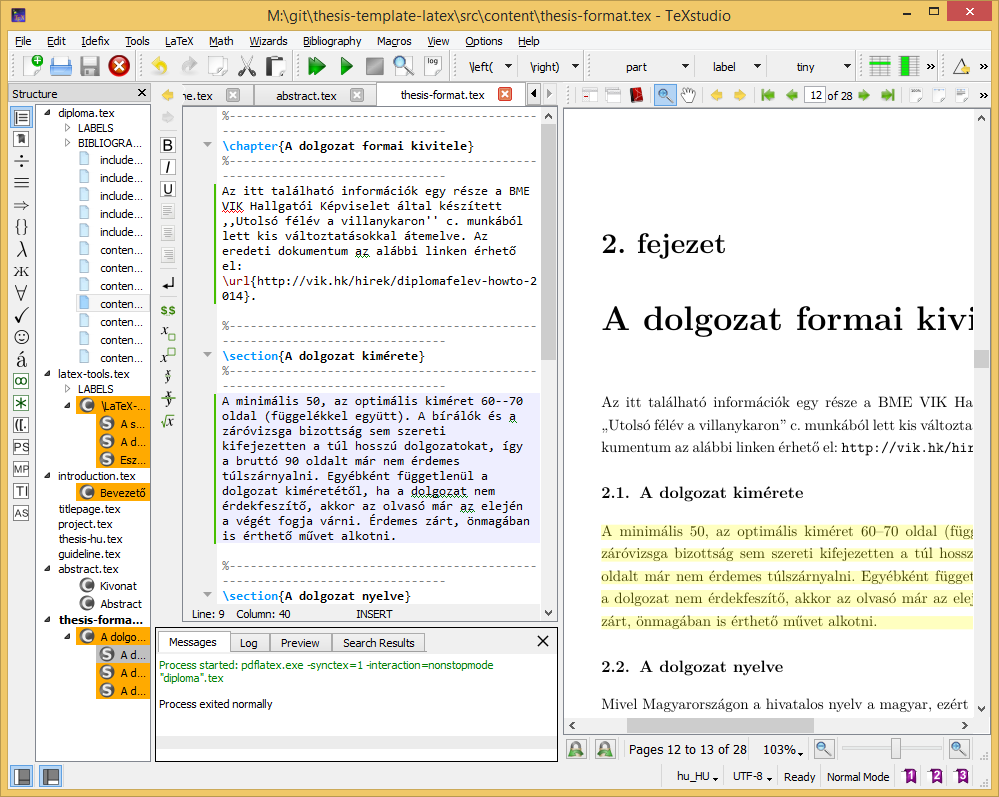
\includegraphics[width=150mm, keepaspectratio]{figures/TeXstudio.png}
\caption{A TeXstudio \LaTeX-szerkesztő.} 
\end{figure}

%----------------------------------------------------------------------------
\clearpage\section{Válasz az ,,Élet, a világmindenség, meg minden'' kérdésére}
%----------------------------------------------------------------------------
A Pitagorasz-tételből levezetve
\begin{align}
c^2=a^2+b^2=42.
\end{align}
A Faraday-indukciós törvényből levezetve
\begin{align}
\rot E=-\frac{dB}{dt}\hspace{1cm}\longrightarrow \hspace{1cm}
U_i=\oint\limits_\mathbf{L}{\mathbf{E}\mathbf{dl}}=-\frac{d}{dt}\int\limits_A{\mathbf{B}\mathbf{da}}=42.
\end{align}


%\label{page:last}
\end{document}
